\title{Blockchain}
\maketitle

\chapter{Introduzione alle Blockchain}

\section{Definizione}

Una blockchain è:
\begin{itemize}
    \item un sistema che si comporta come una terza parte fidata e affidabile, non centralizzata, sempre online, per preservare uno stato condiviso, mediare scambi e fornire computazioni sicure
    \item un \textbf{registro distribuito} che memorizza \textbf{dati di transazioni}, raggruppati in \textbf{blocchi} che costituiscono una lista collegata \textbf{crescente e inalterabile}.
    \item gestita da un grande gruppo di server collegati
\end{itemize}
Altre definizioni inerenti:
\begin{itemize}
    \item \textbf{full node}: memorizzano una copia della intera blockchain e possono creare blocchi. Rappresentano una minoranza.
    \item \textbf{consenso (consensus)} tra full nodes: hanno gli stessi blocchi, sono tutti d'accordo e non ci sono incoerenze sulla blockchain
    \item \textbf{wallet}: software per fare delle transazioni e per verificare la loro validità, usando la crittografia asimmetrica. La chiave pubblica identifica l'utente.
    \item \textbf{public = permissionless}: chiunque può essere un utente o partecipare con un full node, eseguire transazioni, partecipare al processo di consenso che definisce la evoluzione della blockchain
    \item \textbf{private = permissioned}: blockchain operate da entità riconosciute, full node identificabili e ci sono regole per l'accesso. Il \textbf{consortium} è un caso speciale di blockchain permissioned perchè è operata da più entità riconsciute. 
\end{itemize}

\section{Rete P2P}
I full node collaborano al mantenimento di una rete peer$-$to$-$peer per scambio di blocchi e transazioni. Molti wallet usano questo protocollo per connettersi ai full node. Il funzionamento della blockchain è indipendente dal protocollo specifico usato infatti capita spesso che, in corrispondenza di un aumento di utilizzo della bc, ci sia un cambio di protocollo usato, in modo da soddisfare meglio le richieste dipendenti dall'utilizzo. I full node possono reti e protocolli alternativi come l' \textbf{high-speed block relay network} usato dai miners e il \textbf{dedicated transaction information servers} usato da alcuni programmi di wallet. 

Quando eseguiti per la prima volta, i programmi non conoscono nessun indirizzo IP di full node attivi. Per scoprirli devono rivolgersi a degli specifici server chiamati \textbf{DNS seeds}. La risposta include uno o più \textbf{DNS A records} (I record DNS sono l'entità più piccola che contiene l'informazione esatta relativa "all'appartenenza" di un determinato dominio a un indirizzo di destinazione) con gli indirizzi IP dei full node che potrebbero accettare nuove connessioni in arrivo.\\

Prima che un full node possa validare una transazione non confermata e i blocchi minati di recente, deve scaricare e validare tutti i blocchi a partire da quello numero 1. Quel blocco è chiamato \textbf{Initial Block Downlaod (IBD)} o initial sync. Il blocco numero 0 si chiama \textbf{genesis block} e contiene transazioni iniziali che rappresentano tipicamente la nascita della blockchain e la distribuzione iniziale della criptovaluta associata alla blockchain, ad esempio. Contiene informazioni riguardo i primi fullnode e la quantità di moneta virtuale esistente all'inizio e come viene distribuita.\\

\textbf{Block broadcasting}: azione eseguita quando un miner scopre un nuovo blocco che consiste nel mandare in broadcast il blocco stesso ai suoi vicini peers (neighbors). Esiste, in modo analogo, anche la \textbf{Transaction broadcasting}. 


\section{Coin vs Token}
Parlando di \textbf{criptovalute} associate alle blockchain, dobbiamo distinguere tra:
\begin{itemize}
    \item \textbf{coin}: unità della valuta virtuale della blockchain, usata per le transazioni
    \item \textbf{token}: unità secondarie che risiedono nella blockchain con svariati scopi. Esistono due tipologie di token:
    \begin{itemize}
        \item \textbf{utility token}: rappresenta il diritto a ottenere prodotti o servizi da un emettitore di token, come se fossero dei veri e propri buoni
        \item \textbf{security token}: asset digitale il cui valore deriva da un asset negoziabile; successivamente, è soggetto alle leggi del governo. Associabili a beni commerciali come se fossero delle azioni. Sono molto preziosi, potrebbero rappresentare ad esempio il diritto di scelta nelle decisioni sulla blockchain usata da una applicazione.\\
        
        \emph{A security token represents traditional, private security interest.
It could represent a share in a company, an LP interest in a fund
or a trust, a member share in an LLC. Essentially, you’re taking
something that today you have on paper and you’re putting an
electronic wrapper around it.}
    \end{itemize}
\end{itemize}


\section{Transazioni}
Le transazioni descrivono pagamenti per beni e servizi, attraverso l'uso di coins. Le parti in gioco sono identificate dalle loro chiavi pubbliche. Ogni pagamento deve essere firmato digitalmente. 


\section{Bitcoin}
Il genesis block risale al 2009. Di solito con Bitcoin si indica la blockchain mentre con bitcoin si indica il coin associato a Bitcoin e si scrive come BTC. Un BTC è formato da parti più piccole, chiamate satoshi, secondo la relazione: 1 BTC $= 10^8$ satoshi. 

Il software \textbf{Bitcoin Core} include un motore di verifica di transazione e si connette alla rete come un full node. \\

La valuta virtuale basata sulla blockchain è tipicamente generata in un processo decentralizzato e competitivo, cioè il \textbf{mining}. I miners di bitcoin sono full node che elaborano transazioni e rendono sicura la rete usando hardware specializzato. In cambio collezionano nuovi bitcoin. Ovviamente il valore di questi bitcoin che ricevono è maggiore di quello associato all'energia usata per effettuare i processi. Tuttavia, questa ricompensa tende a diminuire col tempo poichè non possono essere creati troppi coin perchè ciò corrisponderebbe a una perdita del valore nel mercato. Si pensa inoltre che il meccanismo che usa costruire blocchi sia superato, sfrutta il concetto di meritocrazia in base al lavoro fatto, all'energia spesa.

C'è un \textbf{numero limitato di bitcoin in circolazione} e nuovi bitcoin sono creati a un ritmo prevedibile e decrescente. Vuol dire che la domanda deve seguire i livelli di inflazione per mantenere il prezzo stabile. Dal momento che Bitcoin è ancora un mercato relativamente piccolo rispetto a quello che potrebbe diventare, non è necessaria una grande somma di denaro per muovere il prezzo mercato su o giù e quindi \textbf{il prezzo di bitcoin è ancora molto volatile}. 

\subsection{Transazioni in Bitcoin}
\begin{center}
    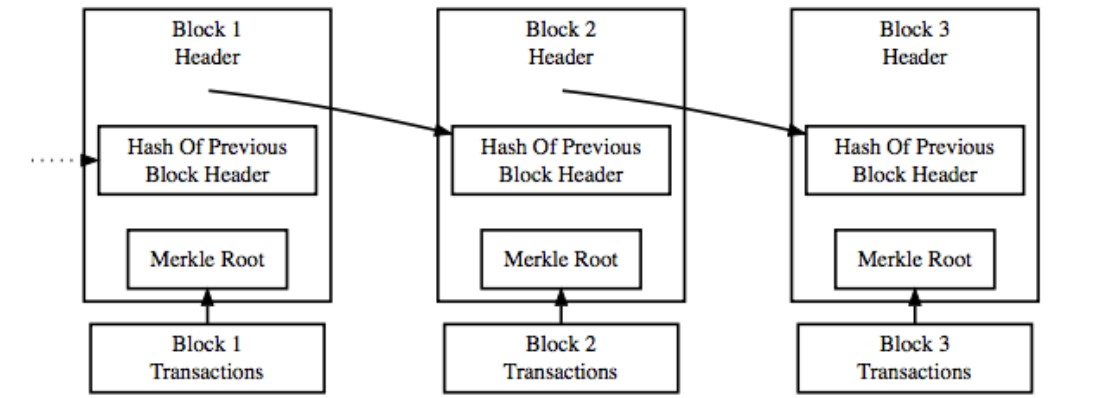
\includegraphics[scale=0.4]{Images/Blockchain/BlocchiBitcoin.jpg}
\end{center}
Viene calcolato l'hash di tutte le transazioni associate ad ogni blocco in un \textbf{Merkle Tree}, finchè un hash unico, la \textbf{Merkle Root}, non è prodotto e memorizzato nell'header di un blocco, insieme all'hash dell'header del blocco precedente. 

\subsubsection{Merkle Tree}
\begin{center}
    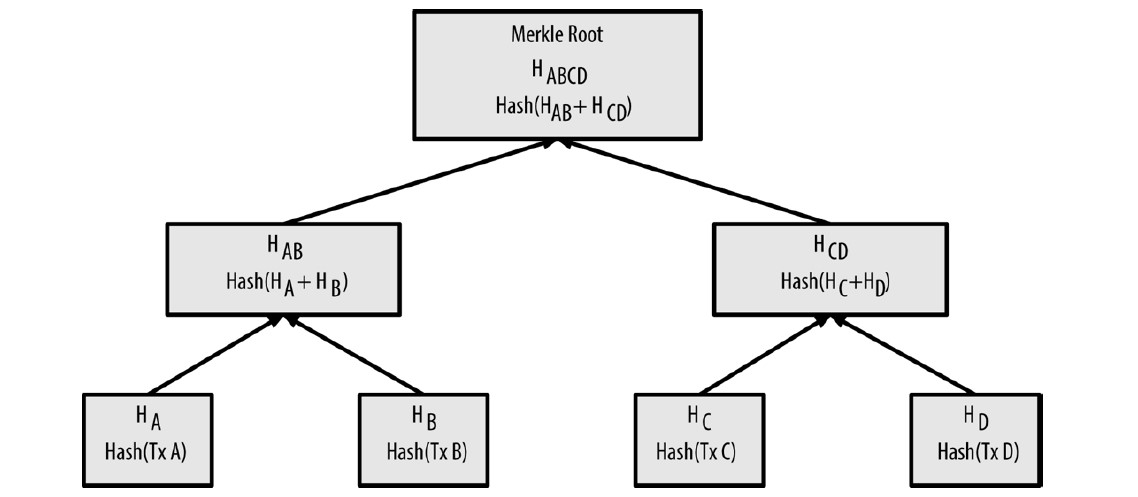
\includegraphics[scale=0.4]{Images/Blockchain/MerkleTree.jpg}
\end{center}

Un Merkle Tree è costruito facendo l'hash dei dati accoppiati (le foglie), e poi accoppiando e facendo l'hash dei risultanti finchè non si ottiene un hash unico, la Merkle Root.\\

Le transazioni in Bitcoin sono collegate insieme e hanno:
\begin{itemize}
    \item \textbf{input}: riferimento ad un output di una transazione precedente
    \item \textbf{output}: quantità di valuta virtuale da trasferire
\end{itemize}
In particolare, le transazioni, potranno avere uno o più input e uno o più output. Se l'output è maggiore del totale degli input, la transazione non è valida. Ad esempio, se Alice vuole spendere 1 BTC bisogna vedere le transazioni passate per capire se può permetterselo. Per validare una transazione bisogna ricostruire tutto il percorso delle transazioni precedenti di quell'utente. Con un'unica lettura non si può sapere di quanto dispone qualcuno, non c'è un "conto". Se l'input è 50 ma si vogliono mandare solo 25, vengono generati due output, uno da 25 per il ricevente e un altro, sempre da 25, per lo stesso mittente.

Nella pratica il ricevitore manda la sua chiave pubblica al pagante il quale crea la transazione, specificando l'ouput e la "signature script" che include l'hash della chiave pubblica del ricevitore. Il pagante firma la transazione con la sua chiave privata. A tal proposito ricordiamo che la firma digitale dipende anche dal contenuto, non solo dalla chiave. La transazione viene mandata dal pagante alla rete di full node i quali verificano ed eventualmente aggiungono la transazione alla blockchain.


\section{Smart contract}
Sono dei \textbf{programmi memorizzati nella blockchain} creati con transazioni speciali e forniti con un indirizzo unico. \'E una espressione di logica contrattuale, può implementare \textbf{qualcunque algoritmo} e ha un comportamento deterministico oltre a poter interagire con gli altri smart contract. 

Il programma è accessibile da tutti, ogni volta che ci si interagisce, se ne cambia lo stato il quale è condiviso, in tutte le repliche della blockchain. Una modifica dello stato del programma consiste in una transazione, ogni volta che qualcuno chiede l'esecuzione di un servizio del programma paga, quindi c'è una transazione che viene tracciata e che cambia lo stato.
Lo smart contract expone una interfaccia che indica quali siano i metodi invocabili e i servizi che si possono richiedere. Potrebbe ritornare dei dati o memorizzarli e le interazioni sono basate sullo scambio di messaggi. Esempi di smart contract:
\begin{itemize}
    \item DApp (decentralized application): frontend $+$ decentralized logic (tipo bitTorrent)
    \item ICO (Initial Coin Offering): per crowdfounding per un singolo progetto, in cambio di token specifici dell'ICO
    \item DAO (Decentralized Anonymous Organization): organizzazione autonoma regolata da uno smart contract 
\end{itemize}

Ci sono similarità tra i comportamenti multi$-$transazionali degli smart contract nelle criptovalute come Ethereum e i classici problemi di concorrenza nella memoria condivisa. 
\begin{itemize}
    \item \textbf{Analogia contracts-as-concurrent-objects}: gli account che usano gli smart contract nella blockchain sono come i thread che usano oggetti concorrenti nella memoria condivisa
    \item relazione tra i comportamenti osservabili di contratto e i temi di concorrenza ben conosciuti, come l'atomicità, interferenza, sincronizzazione, proprietà di risorse.
\end{itemize}


\section{Ethereum}
Obiettivo: fornire un World Computer (computer mondiale) flessibile, condiviso e sicuro. Corrisponde a un sistema distribuito e replicato. Ethereum permette agli sviluppatori di programmare e distribuire \textbf{smart contract} sulla blockchain per permettere transazioni complesse che vanno molto oltre il semplice trasferimento di valuta virtuale. La criptovaluta è l'ether, si indica con ETH e può essere divisa in parti più piccole: 1 ETH $= 10^9$ GWei $= 10^{18}$ Wei.  \\

Il wallet più usato per interagire con ethereum si chiama \textbf{parity}. Esistono diverse implementazioni del protocollo Ethereum che significa che si possono avere dei full node sviluppati con linguaggi di programmazione diversi ma l'importante è che tutti realizzino lo stesso protocollo di comunicazione e di funzionamento. Una implementazione molto efficiente si chiama \textbf{Geth} che è stata implementata col linguaggio Go.\\

Anche in Ethereum c'è una quantità di denaro limitata, il numero di ether e il tasso di emissione è stato deciso dalle donazioni raccolte nella prevendita del 2014. I risultati erano approssimativamente:
\begin{itemize}
    \item \textbf{60 milioni di ether creati per contributori della prevendita}
    \item 12 milioni (20\% dei precedenti) sono stati creati per lo sviluppo fondo, la maggior parte va ai primi contributori e sviluppatori e il restante alla Fondazione Ethereum
    \item La ricompensa corrente per il mining è di \textbf{2 ether per blocco} più \textbf{tutte le transazioni e tasse del gas (gas fees (?)) contenute nel blocco}
\end{itemize}

\subsection{Account Ethereum}
Ci sono due tipi di account:
\begin{itemize}
    \item account normali: controllati da coppie di chiavi pubbliche e private (cioè utenti umani)
    \item account contratto: controllati dai loro codici interni (ad esempio smart contract)
\end{itemize}
Ethereum usa l'\textbf{Elliptic Curve Digital Signature Algorithm (ECDSA)}, con curva ellittica \textbf{secp256k1}, per validare l'origine e l'integrità dei messaggi. Quando viene generato un nuovo account normale sono generate una chiave pubblica da 512 bit e una privata da 256 bit. L'account non corrisponde direttamente alla chiave pubblica ma agli ultimi 20 bytes del suo hash.

A differenza di bitcoin, che ha solo le transazioni, gli account in ethereum hanno a disposizione dei balances, ovvero dei conti per vedere i bilanci. 

\subsection{Smart contracts in Ethereum}
Ogni smart contract ha un \textbf{indirizzo unico}, assegnato tramite una \textbf{transazione speciale}. Dopo questa transazione, lo smart contract diventa parte immutabile della blockchain quindi non potrà essere rimosso. Dato che è caratterizzato da metodi, ci sono dei metodi che possono essere utilizzati solo da chi ha sviluppato e installato lo smart contract, potrebbe esserci un metodo che in qualche modo disabilità la sua funzionalità, non lo rende più accessibile.   
L'interazione con lo smart contract avviene tramite scambio di messaggi che devono essere firmati da entrambe le parti (in base a chi invia). \\

Lo smart contract è dotato di uno stato perchè ha delle \textbf{capacità di memorizzazione} delle informazioni, ad esempio si può memorizzare una variabile booleana che, in base al valore, dice se è in funzionamento o meno. Il costo della interazione con lo smart contract è a carico di chi manda la richiesta. Se la richiesta comporta l'inserimento di molti dati nello storage dello smart contract il conto sarà salato. Se invece deve solo elaborare dati, senza memorizzare qualcosa, il costo è tipicamente più basso. \\

Il codice sorgente è scritto con \textbf{Solidity} (simile a Javascript)
\begin{itemize}
    \item compilato in un \textbf{bytecode} di istruzioni di basso livello (opcodes)
    \item eseguito sulla \textbf{Ethereum Virtual Machine (EVM)}
\end{itemize}
Lo stato di Ethereum è una grande struttura di dati che contiene non solo tutto
conti e saldi, ma uno stato della macchina, che può cambiare
da blocco a blocco secondo un insieme predefinito di regole, e
che può eseguire codice macchina arbitrario.
Vengono definite le regole specifiche per cambiare stato da blocco a blocco
dall'EVM.

\begin{itemize}
    \item Kovan, Ropsten: sono delle testnet, ovvero delle blockchain non ufficiali, online, gestite da fullnode ma permettono di fare dei deployment e testing senza spendere nulla
    \item Truffle: framework per lo sviluppo, permette allo sviluppatore di testare gli smart contract su una EVM locale e di rilasciarli su Ethereum o su testnet 
    \item Ganache: permette di creare una blockchain locale, della quale abbiamo completo controllo. 
\end{itemize}


L'esecuzione di qualsiasi metodo ha un costo in termini di Gas (carburante). Operazioni differenti hanno prezzi differenti. 
\begin{center}
    \textbf{TX Fee = Gas used * Gas Price}
\end{center}

\begin{center}
    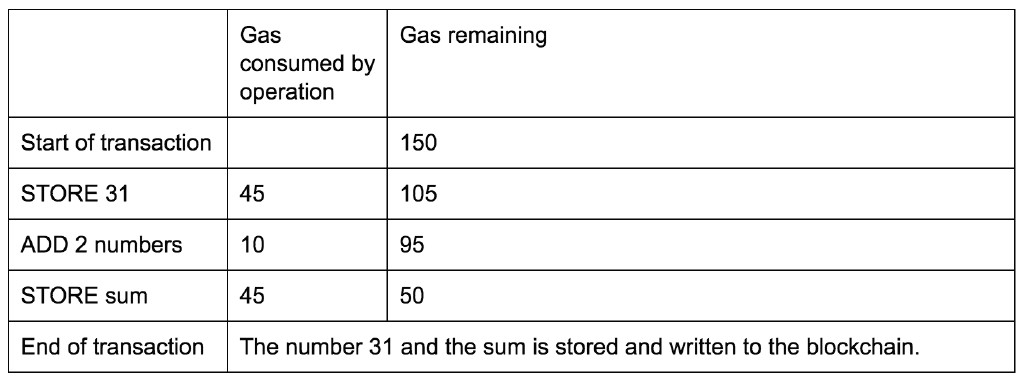
\includegraphics[scale=0.4]{Images/Blockchain/GasPrice.jpg}
\end{center}

STORE, ADD e STORE sono degli opcode e, come si può vedere, ognuno ha un costo. Attenzione che non abbiamo ancora detto il valore di un'unità di carburante perchè non viene deciso da chi sviluppa lo smart contract. Colui che sviluppa lo sc deve cercare di fare il contratto più efficiente possibile, quindi che non abbia codice ridondante che si traduce in opcode in più che hanno un costo. 

Il costo totale della transazione è uguale alla somma del gas usato per gli opcode necessari, moltiplicato per il gas price deciso dal cliente. Il cliente, nel momento in cui richiede l'esecuzione di un metodo, dice quanto è disposto a spendere per unità di carburante, quindi in pratica decide lui il prezzo. 
\begin{itemize}
    \item \textbf{Gas Used}: unità di carburante usate per la transazione
    \item \textbf{Gas Limit}: limite alle unità di carburante che il cliente per i quali è disposto a pagare, non sa quante sono necessarie per la esecuzione del metodo, dovrebbe essere sufficiente
    \item \textbf{Gas Price}: prezzo dell'unità di gas deciso dal cliente. Più è alto il gas price e più velocemente la transazione sarà inclusa nel blocco. Non si ha nessuna garanzia che con un gas price elevato venga inclusa velocemente la transazione
\end{itemize}

Attualmente il gas price medio è di 10 Gwei. Se il gas limit è basso c'è rischio che si vada in \textbf{out of gas} ovvero manca carburante per eseguire la transazione. Il \textbf{Block Gas Limit (BGL)} è il limite della quantità di gas che un blocco può includere. 

Se si mette un gas limit troppo alto si rischia di rendere poco appetibile la transazione per i full node che devono creare i blocchi. Ogni miner, full node che crea il blocco, cerca di massimizzare il proprio profitto blocco per blocco. Nel blocco sappiamo che possono esserci al massimo BGL unità di carburante: l'ideale sarebbe scegliere di mettere nel blocco tutte le transazioni, raggiungendo il limite di carburante BGL, con le transazioni il cui gas price è più alto. Ma il full node, vedendo una richiesta di esecuzione del metodo, non fa il calcolo del gas che verrà usato per eseguire quel metodo, non lo moltiplica per il gas price per sapere quanto guadagnerà perchè sarebbe uno spreco di tempo. Il full node vede arrivare una richiesta che ha un gas limit e un gas price, moltiplica gas price per gas limit e quello per lui è idealmente quello che ricava dall'esecuzione di quella transazione. \'E meglio che un utente metta un gas limit non elevatissimo e un gas price non piccolo, in questo modo avrebbe una transazione con un valore elevato e però, in termini di gas, costa poco. Quella transazione potrebbe valere meno di una con gas price più piccolo e gas limit più grande, però sarebbe comunque preferita dal miner. 


\subsection{Strutture dati Ethereum}
Ci sono molti dati da salvare questo tipo di blockchain: conti degli utenti, stato della blockchain, stato degli smart contract, transazioni. Tutte queste informazioni sono conservate all'interno dei blocchi, viene utilizzata una struttura dati che prende il nome di \textbf{Modified Merkle Patricia Trie}. Molto efficiente e permette ricerche molto veloci.  

\begin{center}
    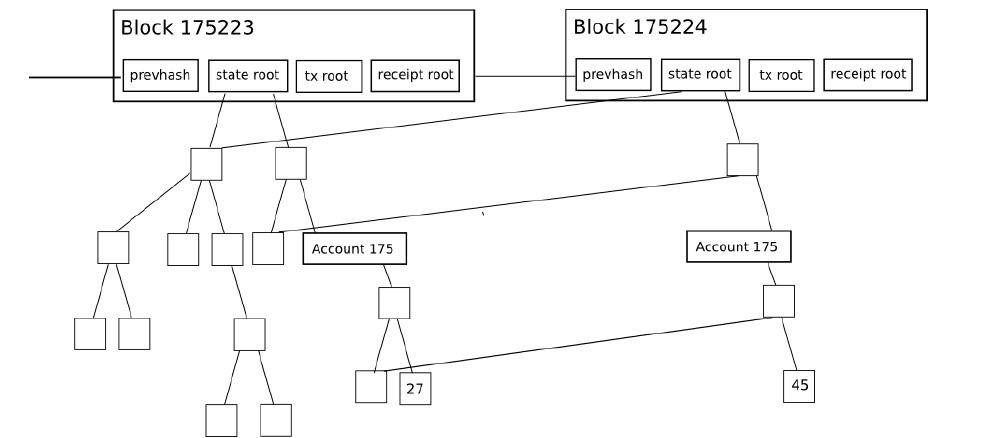
\includegraphics[scale=0.4]{Images/Blockchain/MerkleProofs.jpg}
\end{center}

Sostanzialmente è un insieme di tre alberi:
\begin{itemize}
    \item \textbf{Transaction Tree}: per richieste di transazione
    \item \textbf{Receipt Tree}: memorizza i risultati delle transazioni
    \item \textbf{State Tree}: memorizza lo stato (mappa chiave valore, chiave indirizzo, valore valore conto) degli account
\end{itemize}

\section{Modelli di consenso}
Un modello di consenso è l'insieme delle regole che permette di stabilire quale full node è incaricato di pubblicare il prossimo blocco. Sono di tipo diverso, per adesso abbiamo parlato solo di quelli di merito, basati sulla elaborazione effettuata. 

I più importanti sono associati alle blockchain permissionless. In quelle private invece è più facile creare dei modelli di consenso efficienti perchè di solito si ha un controllo maggiore su chi possiede i fullnode e c'è maggiore fiducia. Ovviamente un motivo per attivare un fullnode è quello economico nel senso che si vuole ottenere una ricompensa che vada non solo a coprire le spese necessarie a competere, ma anche ad andare in positivo. Un altro aspetto è la fiducia reciproca, non possiamo assumere che ci sia fiducia tra uno e l'altro all'interno della blockchain. \\

Tutti i modelli di consenso partono dalla assunzione che esiste un blocco iniziale sul quale sono tutti d'accordo (il genesis block). Gli utenti seguono il modello di consenso secondo il quale i blocchi sono aggiunti al sistema. La catena di blocchi, sfruttando gli hash, rende difficile la modifica di un blocco. Gli utenti validatori possono validare ogni blocco singolarmente. Principali modelli di consenso, ciascuno rappresenta una famiglia di protocolli:
\begin{itemize}
    \item Proof of Work: prova del lavoro svolto (Bitcoin, Ethereum) [reti pubbliche]
    \item Proof of Stake: quello a cui vuole passare Ethereum, usato da Algorand [reti pubbliche]
    \item Round Robin [reti private]
    \item Proof of Authority / Proof of Identity [reti private]
    \item Proof of Elapsed Time [reti private]
\end{itemize}

\subsection{Proof of Work}
La competizione tra full node si basa sulla elaborazione di un compito moderatamente complessa, la singola elaborazione non è difficile però tipicamente bisogna ripetere molte volte l'operazione. Ogni operazione deve essere verificabile. Richiede hardware specializzato, ASIC: Application$-$Specific Integrated Circuit.

In generale bisogna calcolare l'\textbf{hash} di alcuni dati includendo un elemento pseudocasuale. Tipicamente i dati sono le transazioni da inserire nel blocco. Bisogna ripetere l'operazione di hash finchè, includendo un certo valore pseudocasuale, il risultato ottenuto non è minore di una \textbf{soglia}. Gli altri full node verificheranno che sia soddisfatta questa richiesta ricevendo le transazioni e il valore pseudocasuale usato. Se il timestamp della mia firma è precedente a quello degli altri che hanno fatto questo calcolo, vinco io e il mio blocco diventa blocco ufficiale della blockchain e ricevo un premio in termini di coin. La soglia varia ogni tot blocchi per garantire che il tempo di calcolo resti in media uguale e è parte del modello di consenso, ci si mette d'accordo tutti.  

\subsubsection{PoW in Bitcoin}
Viene usata la funzione SHA256 per calcolare l'hash e le viene data in input: la Merkle Root, l'header del blocco precedente e il random nonce. Si ripete cambiando il nonce finchè non siamo sotto soglia. La soglia viene valutata ogni 2016 considerando il tempo medio utilizzato per la generazione di quel numero di blocchi.

\subsubsection{PoW in Ethereum}
Si basa su un algoritmo che si chiama \textbf{Ethash}. Usa la funzione di hash Keccak$-$256 e combina un nonce casuale, l'hash dell'header del blocco precedente e alcuni elementi di dati presi dall'insieme delle transazioni. Concetto della soglia uguale.\\

Contro il Proof of Work l'attacco più grave è chiamato \textbf{51\% Attack} in cui un insieme di persone che possiedono dei full node hanno la maggioranza della potenza di calcolo (\textbf{hash rate}) dell'intera rete dei fullnode. Permetterebbe di riscrivere la storia della blockchain. \\

Una cosa che capita non raramente è la \textbf{fork} e ciò avviene quando ci sono due full node che contemporaneamente riescono a creare il nuovo blocco. Dato che nessun full node è connesso completamente al resto della rete, ma ne conosce solo alcuni succede che metà sono d'accordo con uno e metà con un'altro. Magari la catena intanto va avanti. 

\begin{center}
    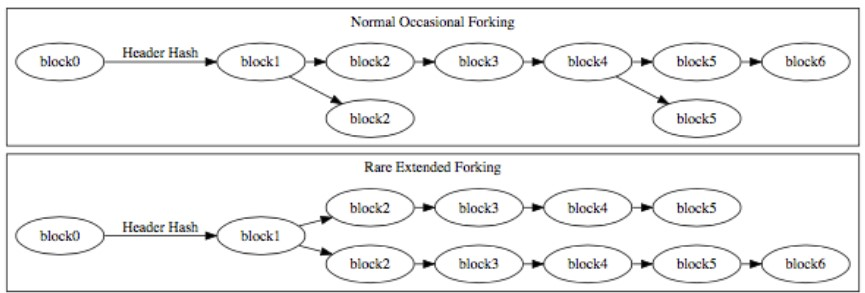
\includegraphics[scale=0.4]{Images/Blockchain/ProofOfWork.jpg}
\end{center}

La seconda versione sotto è più rara ma dipende in realtà può succedere se alcuni full node sono in coalizione e collaborano tra di loro, tenendo nascosto il ramo che stanno sviluppando. Una volta che il loro ramo diventa più lungo di quello originale, lo pubblicano, gli altri nodi, vedendo che esiste un ramo molto più lungo di quello che conoscono già, abbandonano quello originale e si "attaccano" a quello nuovo. \\

La PoW ha un dispendio energetico molto grande, i full node sono tipicamente server o cluster specializzati e potenti.

\begin{center}
    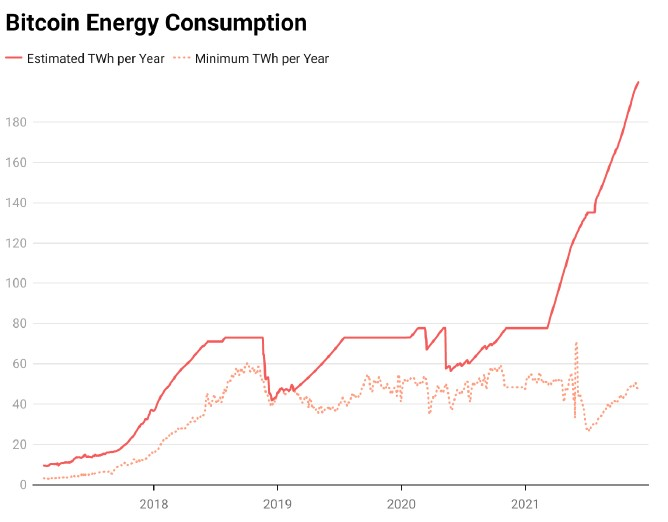
\includegraphics[scale=0.4]{Images/Blockchain/BitcoinEnergyConsumption.jpg}
\end{center}


\subsection{Proof of Stake}
Si basa su dei protocolli che servono a mettere d'accordo le parti e garantire che prima o poi tutti possano produrre blocchi, premiando comunque chi si comporta meglio. Il meccanismo è quello della \textbf{elezione}, tutti i full node si candidano per creare il blocco ma solo uno viene eletto. Non tutti hanno la stessa probabilità, viene aumentata per chi mette in gioco più risorse non di calcolo, ma di denaro, \textbf{stake}. Lo stake è una quantità di crittovaluta che io metto in gioco, non lo spendo e lo metto come garanzia di buon comportamento. Se mi comporto male e mi scoprono, gli altri hanno il diritto di prendere il mio stake e spartirselo. 

Vantaggi:
\begin{itemize}
    \item Riduco rischi centralizzazione: tutti hanno la possibilità, non solo i più "forti"
    \item Efficienza energetica
\end{itemize}
Svantaggi:
\begin{itemize}
    \item L'elezione dei partecipanti richiede \textbf{casualità} ed è difficile ottenerla
    \item Possibili attacchi sferrati in maniera più semplice
\end{itemize}


Un nodo non può generare numeri casuali, perchè potrebbe fare il suo comodo. Una sorgente di casualità è la blockchain stessa quindi potrei calcolare l'hash della blockchain esistente, evolvendo nel tempo cambia periodicamente. Non va bene perchè un nodo può decidere che transazioni mettere nel blocco quindi potrebbe attuare questa scelta in modo che sia sempre lui a dover creare il blocco. Questo si chiama \textbf{grinding attack}. 

Si usano dei protocolli distribuiti o per decidere chi è il prossimo full node autorizzato a creare il blocco o per mettere d'accordo tutti i full node sulla struttura del prossimo blocco. Viene definito da tutti i full node insieme interagendo tra di loro.

\subsubsection{Eventual-consensus PoS protocols}
Rappresenta la prima casistica sopra, si sorteggia un full node che diventa quello autorizzato a creare il nuovo blocco. Più un blocco invecchia e più è considerato solido. Viene usato in \textbf{Ouroboros, Snow White, Ouroboros Praos e Ouroboros } con garanzie rigorose e da Peercoin e NXT in the wild, ovvero che non c'è nessuna verifica della correttezza matematica di quei protocolli.

\subsubsection{Blockwise-BA PoS protocols}
Rappresenta la seconda casistica, tutti i full node danno un contributo. Utilizzato da \textbf{Algorand} con garanzie rigorose e \textbf{Casper} (usato in Ethereum 2.0) in the wild.

\subsubsection{Nothing at Stake problem}
A differenza Proof of Work, in cui serve grande potenza di calcolo per minacciare la sicurezza della blockchain, nella Proof of Stake non serve disporre di tanta potenza per creare eventuali problemi.
Un attacco possibile è il nothing ad stake attack. 


\subsubsection{Long-range attacks}
Un insieme di full node che si coalizzano per l'attacco creano un ramo della blockchain per conto loro e lo tengono nascosto. Lo renderanno pubblico solo nel momento in cui sarà più lungo di quello corretto in modo da convincere i full node che il loro sia quello originale. Di solito si applica usando anche l'identità rubata di alcuni full node che hanno partecipato in passato e che ora sono offline. Ci sono due classi di longrange attacks:
\begin{itemize}
    \item \textbf{posterior corruption}: gli avversari mantengono le chiavi segrete di account con pochi stake, la densità dei blocchi generati potrebbe essere indistinguibile da quella generata in modo onesto
    \item \textbf{stake-bleeding}: l'avversario attua l'attacco facendo leva
commissioni di transazione utilizzate come ricompensa per l'esecuzione del protocollo PoS
\end{itemize}

\subsubsection{Come mitigare gli attacchi long-range}
\begin{itemize}
    \item \textbf{checkpoint}: solo gli ultimi k blocchi possono essere riorganizzati
    \item \textbf{crittografia con evoluzione delle chiavi}
    \item \textbf{statistiche rigorose sulla densità della catena}
\end{itemize}



\subsection{Round Robin}
Usato da qualche rete permissioned. I nodi \textbf{prendono un turno} nel creare i blocchi. C'è un \textbf{timeout} per evitare che i blocchi non attivi fermino il processo di crescita della blockchain. Manca di enigmi crittografici e richiede poca potenza.

\subsection{Proof of Authority/Proof of Identity}
I nodi che pubblicano devono avere \textbf{le loro identità verificabili e provate} all'interno della rete della blockchain. I nodi che pubblicano hanno una \textbf{reputazione} da preservare e migliorare. Minore è la reputazione e minore sarà la probabilità di pubblicare un blocco. Si applica solo a reti permissioned. 

\subsection{Proof of Elapsed Time}
Ogni nodo di pubblicazione richiede un tempo di attesa da una fonte di tempo hardware sicura all'interno del proprio sistema informatico. L'origine dell'ora hardware sicura genererà un'\textbf{attesa casuale}
volta. I nodi di pubblicazione prendono il tempo casuale che gli viene assegnato e
diventano inattivi per quella durata. Una volta che un nodo di pubblicazione viene riattivato dallo stato inattivo, crea e pubblica un blocco sulla rete blockchain. Qualsiasi nodo di pubblicazione ancora inattivo smetterà di attendere e l'intero processo ricomincia. Richiede un ambiente di esecuzione autorizzato e affidabile.





\section{Blockchain simili alle funzioni di hash di Merkle}
La struttura di una blockchain è molto simile a quella dello schema di Merkle per le funzioni di hash, dove una funzione di compressione è iterata su un messaggio che è elaborato in blocchi:
\[
m = {m_1, \dots, m_n} \hspace{1cm} H(m) = h_n = H(m_n, h_{n-1}) \hspace{1cm} h_1 = H(m_1)
\]
Le funzioni di hash di Merkle sono necessarie per soddisfare 3 differenti proprietà di sicurezza al alto livello:
\begin{itemize}
    \item resistenza della preimmagine: dato h, difficile trovare x se H(x) $=$ h
    \item resistenza alla seconda preimmagine: dato x$_1$ difficiel trovare x$_2$ tale che h$_1 = $ h$_2$
    \item resistenza alle collisioni: difficile trovare x$_1$ e x$_2$ tali che h$_1 = $ h$_2$
\end{itemize}
La seconda preimmainge è qualcosa che le blockchain non dovrebbero avere. Tuttavia, i checkpoint sono obiettivi importanti per attacchi che sfruttano la seconda preimmagine. In \textbf{scale temporali molto lunghe} tale debolezze dovrebbero essere considerate.

\section{Attacchi esclissi (ecplise)}
Gli attacchi eclipse operano al livello di \textbf{rete peer-to-peer}. Un nodo sotto attacco ottiene una vista distorta della blockchain, visto che l'avversario controlla i canali di comunicazione e applica filtri a messaggi scambiati con gli altri nodi.

\section{Riepilogo delle possibili violazioni della sicurezza}
\begin{itemize}
    \item PoW: attacco del 51\%
    \item PoS: Nothing at stake e attacchi Long$-$rage
    \item Problemi generali: attacco della seconda preimmagine e attacchi eclissi
\end{itemize}


